\documentclass[a4paper,10pt]{article}

\usepackage[english]{babel}
\usepackage[utf8]{inputenc}
\usepackage{titlesec}
\usepackage{graphicx}
\usepackage{mathtools}
\usepackage{amsthm}
\usepackage{amsfonts}
\usepackage[top=1.0in,bottom=1.0in]{geometry}
\usepackage{hyperref}
\usepackage[singlelinecheck=false]{caption}
\usepackage[backend=biber,url=true,doi=true,eprint=false,style=alphabetic]{biblatex}
\usepackage{enumitem}
\usepackage[x11names, rgb]{xcolor}
\usepackage{tikz}
\usepackage[justification=centering]{caption}
\usepackage{indentfirst}
\usepackage{abstract}
\usepackage[titletoc]{appendix}
\usepackage{bookmark}
\usepackage{minted}
\usepackage{algorithm}
\usepackage{algpseudocode}

\usetikzlibrary{snakes,arrows,shapes}

\addbibresource{../common/references.bib}

\newcommand\blfootnote[1]{%
  \begingroup
  \renewcommand\thefootnote{}\footnote{#1}%
  \addtocounter{footnote}{-1}%
  \endgroup
}

\DeclareMathOperator*{\argmin}{arg\,min}
\DeclareMathOperator*{\argmax}{arg\,max}

\newcommand\defeq{\mathrel{\overset{\makebox[0pt]{\mbox{\normalfont\tiny\sffamily def}}}{=}}}

\renewcommand{\abstractnamefont}{\normalfont\Large\bfseries}

\algrenewcommand\algorithmicrequire{\textbf{Input}}
\algrenewcommand\algorithmicensure{\textbf{Output}}

\titleformat{\section}
  {\normalfont\scshape\bfseries}{\thesection}{1em}{}
\titleformat{\subsection}
  {\normalfont\scshape\bfseries}{\thesubsection}{1em}{}
\titleformat{\paragraph}
  {\normalfont}{\theparagraph}{1em}{}
\titleformat{\subparagraph}
  {\normalfont}{\thesubparagraph}{1em}{}

\captionsetup[table]{labelsep=space}

\theoremstyle{plain}

\newtheorem*{spn-def}{Definition}
\newtheorem*{spn-thm}{Theorem}

\setlength{\parskip}{1em}

\begin{document}

\begin{titlepage}
  \begin{center}
    \LARGE
    \textbf{An Introduction to Sum-Product Networks}

    \vspace{1.7cm}
    \Large
    A collection of studies on properties, structure, inference and learning on Sum-Product
    Networks

    \vspace{1.7cm}
    \large
    Student: Renato Lui Geh

    Supervisor: Denis Deratani Mauá (DCC IME-USP)
    \vfill
    \large
    University of São Paulo / Universidade de São Paulo (USP)

    Institute of Mathematics and Statistics / Instituto de Matemática e Estatística (IME)
    \vspace{1.5cm}
  \end{center}
\end{titlepage}

\newpage
\null\vspace{\fill}
\begin{abstract}
  \large
  This work is a collection of ongoing studies I am working on for my undergraduate research
  project on automatic learning of Sum-Product Networks. The main objective of this work is logging
  my study notes on this subject in an instructive and uncomplicated way. Most scientific papers
  are cluttered with intricate names and require extensive background on the subject in order for
  the reader to understand what is going on. In this paper we seek to provide an easy reference and
  introductory reading material to those who intend to work with Sum-Product Networks.

  This study is divided into five main sections. We start with an introductory section regarding
  probabilistic graphical models and why Sum-Product Networks are so interesting. Next we talk
  about the structure of the model. Then we analyse some properties and theorems. After that, we
  look on how to perform exact tractable inference. And finally we take a look at how to perform
  learning.

  At the end of this work I include a list of subjects I intend to study. They may include both
  new things as well as already included subjects that I plan on studying further. Since this is a
  work in progress (and in fact will be for the entirety of my undergraduate studies), some
  sections (or subsections) will be incomplete (or otherwise just not as thoroughly detailed). This
  means new sections and subsections may be added in the (near) future.
\end{abstract}
\vspace{\fill}
\newpage
\large
\tableofcontents
\normalsize
\newpage

\section{Introduction}

Probabilistic graphical models can compactly represent many distributions of probability. However,
exact inference in most of them is intractable and models that can compute exact inference in
tractable time are quite limited in compactly representing distributions. An alternative to this
are the use of deep architectures that use multiple hidden variables to increase the compactness
of graphical models, but makes inference in them even more difficult.

In 2011, Poon and Domingos introduced sum-product networks (SPNs). Adding new layers to this new
class of deep architecture not only increases its expressivity but also retains its tractability.
Compared to other tractable models, sum-product networks have shown to be more general
\cite{poon-domingos} and easier to perform learning and inference. Experiments have shown promising
results, with SPNs performing better and faster than other graphical models in vision problems.

In this paper, we show what an SPN is, its properties and how to perform inference and learning on
it.

\section{Structure of Sum-Product Networks}

We will base this section on the works of Poon and Domingos on their article \textit{Sum-Product
Networks: A New Deep Architecture}~\cite{poon-domingos} and also on Gens and Domingos'
\textit{Learning the Structure of Sum-Product Networks}~\cite{gens-domingos}.

\subsection{Partition function}

Probabilistic graphical models represent distributions compactly through a normalized product of
factors.

\begin{equation*}
  P(X=x) = \frac{1}{Z}\prod_k \phi_k (x_{\{k\}})
\end{equation*}

This equation states that the probability of $X$ taking value $x$ is the product of all factors,
with each factor taking a subset of the variables, divided by a partition function. The partition
function is the result of all the product of factors summed out.

\begin{equation*}
  Z = \sum_{x\in \mathcal{X}} \prod_k \phi_k(x_{\{k\}})
\end{equation*}

However, this form cannot represent all distributions. Additionally, inference is exponential in
scope size in the worst-case and learning takes sample size and time exponential. This is because
the partition function $Z$ is the sum of an exponential number of terms, and since all marginals
are sums of these terms, if $Z$ is tractable, then marginals are also tractable.

Since $Z$ can be computed with only sums and products, we can efficiently compute $Z$ if we
reorganize it using the distributive law into an expression with only a polynomial number of sums
and products~\cite{poon-domingos}. Using this idea and Darwiche's network polynomial
\cite{diff-approach-darwiche}, Poon and Domingos introduce sum-product networks.

\subsection{Definition}

We will define sum-product networks with Boolean variables. For the continuous or multi-valued case
see the properties section. We will use the following notation: sets will be bold fonted (e.g.\ the
set $\mathbf{X}$ of variables); variables are uppercase (e.g. $X_1=1,X_2=0$); instances of
variables are lowercase (e.g. $P(X=x)$); indicators are also lowercase but distinction between the
two will be evident (e.g. $P(x_1,x_2)$ vs $S(x_1,x_2,\overline{x}_1,\overline{x}_2)$).

\begin{spn-def}
  A sum-product network (SPN) is an acyclic digraph. An SPN $S$ over variables $X_1,\ldots,X_n$ has
  leaves as indicators $x_1,\ldots,x_n,\overline{x}_1,\ldots,\overline{x}_n$ and internal nodes as
  sums and nodes in alternating layers. For each edge $(i,j)$ that emanates from a sum node $i$,
  there exists a non-zero weight $w_{ij}$. The value of a sum node $i$ is $\sum_{j\in Ch(i)}
  w_{ij}v_j$, where $Ch(i)$ is the set of children of $i$ and $v_j$ is the value of the node $j$.
  The value of a product node $i$ is $\prod_{j\in Ch(i)} v_j$. The value of an SPN is the value of
  its root.
\end{spn-def}

\begin{figure}[h]
  \captionsetup{justification=centering}
  \centering{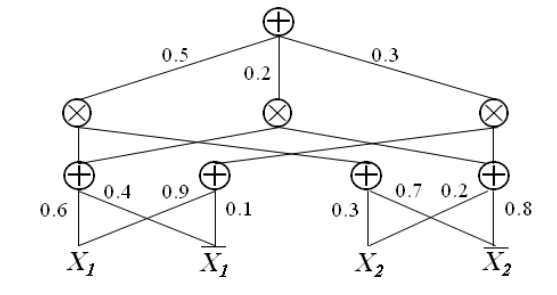
\includegraphics[scale=0.35]{imgs/spn_1.png}
    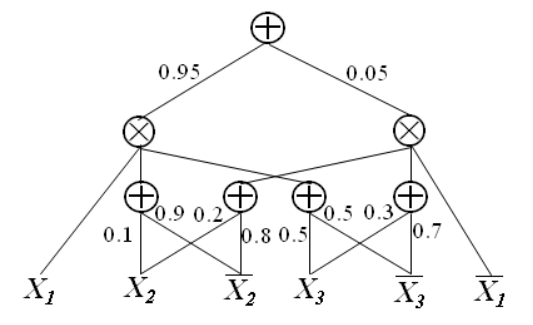
\includegraphics[scale=0.35]{imgs/spn_2.png}
    \caption{Two sum-product networks. The one on the left implements a naive Bayes mixture model
      and the other implements a junction tree. Source:~\cite{poon-domingos}.}
  }
\end{figure}

Sum-product networks are based on network polynomials. The network polynomial of an unnormalized
probability distribution $\Phi(x)\geq 0$ is $\sum_x \Phi(x)\Pi(x)$, where $\Pi(x)$ is the product
of the indicators that have value 1 in state $x$.

The indicators of a variable indicate its value. We will only use Boolean variables for now. A
variable $X_i$ may take values 1 or 0. If $X_i=1$, then the indicators are $x_i=1,\overline{x}_i=0$
and if $X_i=0$ then $x_i=0,\overline{x}_i=1$. If the variable is not instanciated then its
indicators are both set to 1. The indicators of an SPN are consistent with a set if they are set
according to the variables of the set. For example, given the set $\{X_1=1,X_3=0\}$, the indicators
$(x_1,x_2,x_3,\overline{x}_1,\overline{x}_2,\overline{x}_3)$ must be set to $(1,1,0,0,1,1)$.

An SPN $S$ as a function of the indicator variables $x_1,\ldots,x_n,\overline{x}_1,\ldots,
\overline{x}_n$ will be denoted by $S(x_1,\ldots,x_n,\overline{x}_1,\ldots,x_n)$. A complete state
$x$ means that, for each variable $X_i$, there are two possible outcomes for the indicators: either
$x_i=1,\overline{x}_i=0$ or $x_i=0,\overline{x}_i=1$. When an SPN $S$ has a complete state $x$,
instead of enumerating each indicator, we simply abbreviate it to $S(x)$. $S(e)$ will be used to
denote when the indicators are specified according to the evidence $e$. The partition function is
the value of the network polynomial when all indicators are set to 1. If an SPN $S$ has all
indicators set to 1, we refer to it as $S(*)$.

SPNs are defined recursively. The subnetwork $S_n$ rooted at an arbitrary node $n$ in an SPN $S$
is an SPN in itself. Let $\mathbf{X}$ be the set of variables in an SPN $S$, then for all $x\in
\mathbf{X}$ the values of $S(x)$ define an unnormalized probability distribution over $\mathbf{X}$.
The unnormalized probability of evidence $e$ of an SPN $S$ is given by $\Phi_S(e)=\sum_{x\in e}
S(x)$, where the sum is over states consistent with $e$. The $Z$ partition function of a
distribution defined by $S(x)$ is $Z_S=\sum_{x\in \mathbf{X}}S(x)$. The scope of an SPN $S$ is the
set of variables that appear in $S$. A variable $X_i$ is negated in $S$ if $\overline{x}_i$ is a
leaf and non-negated if $x_i$ is a leaf.

The normalized probability distribution of an SPN $S_n$ is given by $P(x)=S_n(x)/Z_n$.

Taking the SPN on the left in Figure 1 as an example:

\begin{align*}
  S(x_1,x_2,\overline{x}_1,\overline{x}_2)=&\phantom{{} +{}}0.5(0.6x_1+0.4\overline{x}_1)(0.3x_2+0.7\overline{x}_2)+\\
                                           &+0.2(0.6x_1+0.4\overline{x}_1)(0.2x_2+0.8\overline{x}_2)+\\
                                           &+0.3(0.9x_1+0.1\overline{x}_1)(0.2x_2+0.8\overline{x}_2)
\end{align*}

The network polynomial is then:

\begin{equation*}
  \Phi = (0.5\times0.6\times0.3+0.2\times0.6\times0.2+0.3\times0.9\times0.2)x_1x_2+\ldots
\end{equation*}

If we have a complete state $x$ as $X_1=1,X_2=0$ then $S(x)=S(x_1,x_2,\overline{x}_1,
\overline{x}_2)=S(1,0,0,1)$. If the evidence $e$ is $X_1=1$, then, following the consistency rule,
we have that $S(e)=S(1,1,0,1)$. And $S(*)=S(1,1,1,1)$.

\section{Properties of Sum-Product Networks}

We will now discuss a few properties described in Poon and Domingos' \textit{Sum-Product Networks:
A New Deep Architecture}~\cite{poon-domingos} and Gens and Domingos' \textit{Learning the Structure
of Sum-Product Networks}~\cite{gens-domingos}.

We first introduce two properties: completeness and consistency. Then we define validity, a
property that guarantees exact inference in time linear to the size of the SPN's edges. After that
we discuss tractability of the partition function, decomposability and a few other properties.

\subsection{Completeness and consistency}

Let us define the two properties:

\begin{spn-def}
  A sum-product network is complete iff all children of the same sum node have the same scope.
\end{spn-def}

This definition states that the children of a sum node must all be from the same variable.
The trivial case is when all the children of the sum node $i$ are leaves. If $S_i$ is complete,
then all leaves are indicators of a same variable. This is easily extended to the general case,
since if, given a sum node $j$, all $Ch(j)$ are complete then all $S_k\in Ch(j)$ are complete and
thus $S_j$ is complete. If there exists an $S_k\in Ch(j)$ that is incomplete, then $S_j$ is
incomplete.

\begin{figure}[h]
  \centering{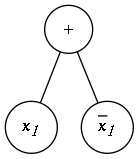
\includegraphics[scale=0.5]{imgs/complete.png}
    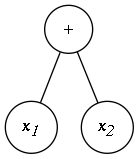
\includegraphics[scale=0.5]{imgs/incomplete.png}
    \captionsetup{justification=centering}
    \caption{On the left a complete SPN\@. On the right an incomplete SPN\@.}
  }
\end{figure}

\begin{spn-def}
  A sum-product network is consistent iff no variable appears negated in one child of a product
  node and non-negated in another.
\end{spn-def}

A variable $X_i$ is negated if there exists a leaf $\overline{x}_i$ on the SPN\@. It is non-negated
if there exists a leaf $x_i$. Therefore, if an SPN $S_k$ has a variable $X_i$, for it to be
consistent $x_i$ and $\overline{x}_i$ cannot appear in more than one child in $S_k$. That leads to
the fact that if an SPN $S_p$ has an inconsistent sub-SPN $S_q$, then $S_p$ is inconsistent.

\begin{figure}[h]
  \centering{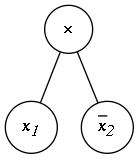
\includegraphics[scale=0.5]{imgs/consistent.png}
    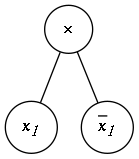
\includegraphics[scale=0.5]{imgs/inconsistent.png}
    \captionsetup{justification=centering}
    \caption{On the left a consistent SPN\@. On the right an inconsistent SPN\@.}
  }
\end{figure}

If an SPN is consistent but incomplete, it does not include monomials that should be present in the
network polynomial and $S(e) \leq \Phi_S(e)$. If the SPN is complete but inconsistent, the
expansion will include more monomials than present in the network polynomial and thus $S(e)\geq
\Phi_S(e)$.

\subsection{Validity}

Validity is an important property in SPNs. Not all SPNs are valid, but validity guarantees
that inference will be exact and tractable.

\begin{spn-def}
  A sum-product network $S$ is valid iff $S(e)=\Phi_S(e)$ for all evidence $e$.
\end{spn-def}

This means that an SPN computes the probability of evidence correctly only if it is valid. Another
important aspect of validity is that, if an SPN $S$ is valid then $S(*)=Z_S$. Validity guarantees
that the probability of evidence will be computed in time linear to the SPN's size. Invalid SPNs
can be used to compute approximate inference.

\begin{spn-thm}
  A sum-product network is valid if it is complete and consistent.
\end{spn-thm}

See~\cite{poon-domingos} for the proof. Completeness and consistency are not necessary for the SPN
to be valid. There are SPNs that satisfy $\Phi_S(e)=\sum_{x\in e}S(x)$ for all evidence $e$, but if
an SPN $S$ is both complete and consistent, then all sub-SPNs of $S$ are valid.

\subsection{Other properties}

\begin{spn-def}
  An unnormalized probability distribution $\Phi(x)$ is representable by a sum-product network $S$
  iff $\Phi(x)=S(x)$ for all states $x$ and $S$ is valid.
\end{spn-def}

This definition states that in all possible states an SPN $S$ will compute the probability of the
state and the partition function correctly.

\begin{spn-thm}
  The partition function of a Markow network $\Phi(x)$, where $x$ is an $n$-dimensional vector, can
  be computed in time polynomial in $n$ if $\Phi(x)$ is representable by a sum-product network with
  a number of edges polynomial in $n$.
\end{spn-thm}

\begin{proof}
  Follows immediately from the definitions of SPN and representability.
\end{proof}

\begin{spn-def}
  A sum-product network is decomposable iff no variable appears in more than one child of a product
  node.
\end{spn-def}

What this definition means is that SPNs are more general than other representations since they do
not require the distribution to be decomposable, unlike arithmetic circuits, mixture models and
junction trees.

If for every sum node $i$ in the SPN $S$, $\sum_{j\in Ch(i)}w_{ij}=1$, then $Z_S=1$ and $P(x)=
S_n(x)$. In this case, for each sum node $i$, we can view $i$ as summing out an implicit hidden
variable $Y_i$ whose values correspond to $Ch(i)$, since summing out a variable means setting all
the indicators concerning the variable to 1, and children of product nodes with values 1 can be
omitted. If $i$ has no parents, then the children's weights are the prior distribution $w_{ij}=
P(Y_i=j)$. If $i$ has parents, then $w_{ij}=P(Y_i=j|\pi_i)$, where $\pi_i$ is the condition that
``on at least one path from $Y_i$ to the root, all of $Y_i$'s ancestors have the values that lead
to $Y_i$ (the ancestors being the hidden variables corresponding to the sum nodes on the path).''
\cite{poon-domingos} If the SPN is also decomposable then the sub-SPN rooted at the $j$-th child
represents the distribution of the variables in it conditioned on $Y_i=j$. See~\cite{poon-domingos}
for more information.


\subsection{Multi-valued discrete variables}

For multi-valued variables, we can simply replace the Boolean indicators $x_i,\overline{x}_i$ with
indicators for the $m$ possible values the variable may take $x_i^1,\ldots,x_i^m$. The multinomial
distribution over $X_i$ would then be written as $\sum_{j=1}^m p_i^j x_i^j$, with $p_i^j=
P(X_i=x_i^j)$.

\subsection{Continuous variables}

We can construct SPNs with continuous variables by assuming variables have an infinite number of
values. The sum of the indicators $\sum_{j=1}^m p_i^j x_i^j$ can be viewed as an integration of the
densities $\int p(x)dx$ with $p(x)$ as the probability density function of $X$\footnote{I plan on
elaborating more on this later.}. For more information see~\cite{poon-domingos}.

\section{Inference on Sum-Product Networks}

As we have seen, inference on SPNs is tractable. In fact, we can compute marginals and MAP in time
linear to the SPN's edges. In this section we will first take a look on how to compute the
probability of a complete state, then we show how to find the marginals of an SPN\@. And finally
we see that computing the MPE is possible my maximizing the nodes.

\subsection{Probability of a complete state}

The complete state $\mathbf{X}$ can be computed by first setting all indicators to be consistent
with the state. For instance, let $\mathbf{X}=\{X_1=1,X_2=0\}$ be the complete state. Then the
indicators are $(x_1,x_2,\overline{x}_1,\overline{x}_2)=(1, 0, 0, 1)$. Computing the probability
of $\mathbf{X}$ is $P(\mathbf{X}=\{X_1=1,X_2=0\})=S(\mathbf{X})/Z$. Assuming our SPN $S$ is valid,
and since for each sum node $i$: $\sum_{j\in Ch(i)} w_{ij}=1=Z_S$, then our probability is
$P(\mathbf{X})=S(\mathbf{X})$ and thus computing the value of the SPN is sufficient.

To compute the value of the SPN we do a bottom-up pass. A bottom-up pass consists of computing all
nodes starting from the bottom and then going up. The trivial case are the leaves. The values of
the leaves are the values of the indicators. In our example, the values of the leaves are
$(x_1,x_2,\overline{x}_1,\overline{x}_2)=(1,0,0,1)$. Consider the SPN on Figure 4. The next nodes
to be computed are sum nodes. The values of the sum nodes are, for each node $i$: $\sum_{j\in
Ch(i)}v_j w_{ij}$. After that we go up a layer again, which in our case means computing the product
nodes: $\prod_{j\in Ch(i)}v_j$, where $i$ is the product node. Finally, once we have the values for
our product nodes we may compute the value of the root node, which is a sum node. The resulting
root node is then the probability of the complete state $\mathbf{X}$ we wanted to find.

\begin{figure}[h]
  \centering{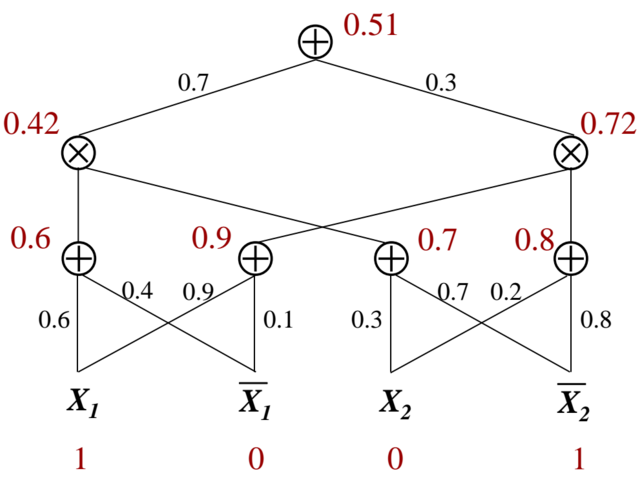
\includegraphics[scale=0.3]{imgs/cstate.png}
    \captionsetup{justification=centering}
    \caption{The value of the probability is  $P(X_1=1, X_2=0)=S(1, 0, 0, 1)=0.51$. Source:
    \url{http://spn.cs.washington.edu/talks/spn11.pdf}.}
  }
\end{figure}

\subsection{Marginals}

Finding marginals is similar to computing the probability of a complete state. However, for
marginals we have unobserved variables.

Take the evidence $\mathbf{e}=\{X_1=1\}$ and the SPN on Figure 5 as example. The variable
indicators are then $(x_1,x_2,\overline{x}_1,\overline{x}_2)=(1,1,0,1)$. Similar to computing the
complete state, we do a bottom-up pass on our SPN, computing the values of each node. Since we
assume the SPN is valid and $Z_S=1$, the resulting marginal is $P(\mathbf{e}=\{X_1=1\})=
S(\mathbf{e})/Z=S(\mathbf{e})=0.69$.

\begin{figure}[h]
  \centering{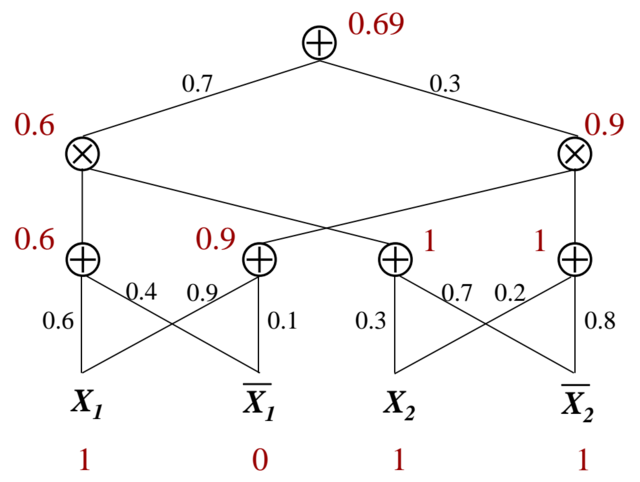
\includegraphics[scale=0.3]{imgs/marginals.png}
    \captionsetup{justification=centering}
    \caption{The value of the marginal is $P(X_1=1)=S(1,1,0,1)=0.69$. Source:
    \url{http://spn.cs.washington.edu/talks/spn11.pdf}.}
  }
\end{figure}

\subsection{Most probable explanation (MPE)}

Computing the MPE of the SPN is similar to computing the MPE on Darwiche's Arithmetic Circuits
\cite{diff-approach-darwiche}: replace all sum nodes with max nodes, do a bottom-up pass to compute
all values of each node and finally do a top-down pass to find the children with max values. The
value of a max node is $\max_{j\in Ch(i)}w_{ij}v_j$, where $i$ is the max node.

Let us take the evidence $\mathbf{e}=\{X_1=1\}$ as an example and compute the MPE state
$\argmax_X P(X|\mathbf{e})$ of the SPN on Figure 6. The indicators given the evidence $\mathbf{e}$
are $(x_1,x_2,\overline{x}_1,\overline{x}_2)=(1,1,0,1)$. Again, we assume that the SPN is valid and
that $Z_S=1$.

First we replace all sum nodes with max nodes. From there we do a bottom-up pass to find all values
of each node. Now, instead of computing the weighted sum on each sum node, we output the max value
weighted on each edge amongst all children on each max node. Since the root of the SPN is now a max
node, the value of the SPN will be the maximum value of all children.

\begin{figure}[h]
  \centering{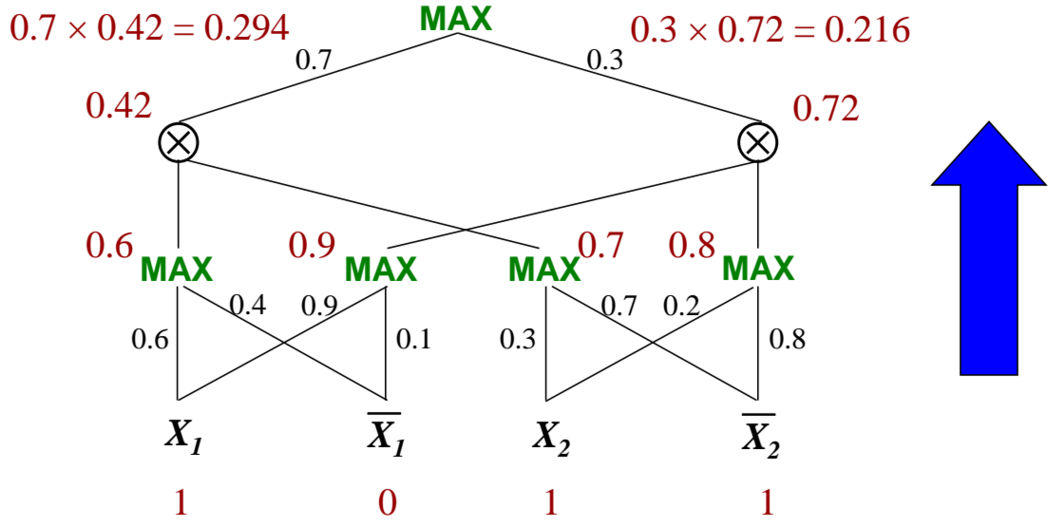
\includegraphics[scale=0.28]{imgs/map_botup.png}
    \captionsetup{justification=centering}
    \caption{A bottom-up pass computes the maximum value a child of the root node may take
    according to its arguments, that is, this pass computes $\max P(X|\mathbf{e})$. Source:
    \url{http://spn.cs.washington.edu/talks/spn11.pdf}.}
  }
\end{figure}

Now we need to get the max variable. We do this by doing a top-down pass and picking the child with
the highest value for each node. Once we reach the leaves we have the $\argmax_X P(X|\mathbf{e})$.

\begin{figure}[h]
  \centering{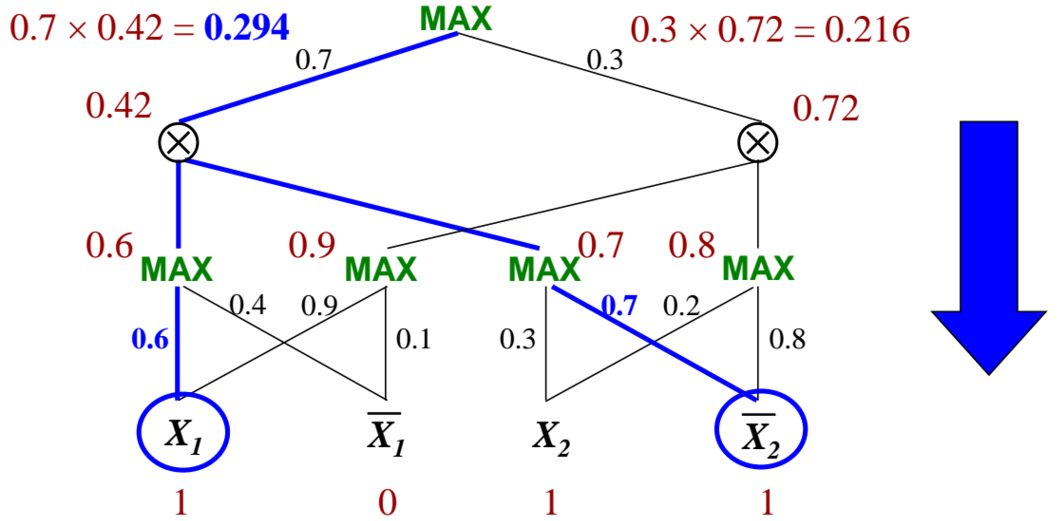
\includegraphics[scale=0.25]{imgs/map_topdown.png}
    \captionsetup{justification=centering}
    \caption{A top-down pass selects the child with the highest value for each node, resulting on
      $\argmax_X P(X|\mathbf{e})$. Source:
      \url{http://spn.cs.washington.edu/talks/spn11.pdf}.}
  }
\end{figure}

By extension of Darwiche's findings on~\cite{diff-approach-darwiche} this procedure will find the
MPE state successfully if the SPN is decomposable or consistent.


\section{Learning Sum-Product Networks}

In this section we are going to show some algorithms on learning Sum-Product Networks.

\subsection{Learning the weights}

This method for learning an SPN was proposed by Poon and Domingos on their article
\textit{Sum-Product Networks: A New Deep Architecture}~\cite{poon-domingos}.

The idea for this learning algorithm is simple: take a valid, dense, and generic SPN, run inference
on it, update weights until convergence and then prune edges that have weight zero and remove
non-root nodes that have no parents. Note that we do not learn the structure of the SPN, but learn
the weights. Algorithm~\ref{pd11-learn}, from Poon and Domingos~\cite{poon-domingos} describes the
learning method.

\begin{algorithm}
  \caption{LearnSPN}\label{pd11-learn}
  \begin{algorithmic}[1]
    \Require Set $\mathbf{D}$ of instances over variables $\mathbf{X}$.
    \Ensure An SPN with learned structure and parameters.
    \State $S \gets $GenerateDenseSPN($\mathbf{X}$)
    \State InitializeWeights($S$)
    \Repeat
    \ForAll{$d\in \mathbf{D}$}
      \State UpdateWeights($S$, Inference($S,d$))
      \EndFor
    \Until{convergence}
    \State $S \gets $PruneZeroWeights(S)
    \State \textbf{return} $S$
  \end{algorithmic}
\end{algorithm}

Although the idea illustrated in Algorithm~\ref{pd11-learn} is simple, creating the starting SPN is
not easy. The SPN must be complete and consistent to be flexible and correct when representing the
training set. Poon and Domingos suggest a general scheme for producing the initial
SPN\@:

\begin{enumerate}
  \item Select a set of subsets of the variables.
  \item For each subset $R$:
  \begin{enumerate}[label*=\arabic*.]
    \item Create $k$ sum nodes $S_1^R,\ldots,S_k^R$.
    \item Select a set of ways to decompose $R$ into other selected subsets $R_1,\ldots,R_l$.
    \item For each of these decompositions:
    \begin{enumerate}[label*=\arabic*.]
      \item For all $1\leq i_1,\ldots,i_l\leq k$:
      \begin{enumerate}[label*=\arabic*.]
        \item Create a product node with parents $S_j^R$ and children $S_{i_1}^{R_1},\ldots,
          S_{i_l}^{R_l}$.
      \end{enumerate}
      \item EndFor
    \end{enumerate}
  \item EndFor
  \end{enumerate}
  \item EndFor
\end{enumerate}

If we assume that we always select a polynomial number of subsets of the variables, and for each of
these subsets we only choose a polynomial number of decompositions, then the SPN is guaranteed to
have a polynomial size and therefore is efficient during the learning and inference passes after
we run Algorithm~\ref{pd11-learn}.

After we create the initial SPN, we now need to initialize the weights. It is evident that we need
not concern too much on the values of these initializations, since on the next steps we will be
performing weight updating. It is a good idea to have all weights of a same sum node initialized
uniformally to avoid bias.

For weight updating, we may either use Gradient Descent or Expectation-Maximization.

For gradient descent, Computing the partial derivative of the SPN $S$ with respect to the weights
can be done by computing the inference of the marginal. Let $n_j$ be the child of the sum node
$n_i$. Then:

\begin{equation*}
  \frac{\partial S(x)}{\partial w_{ij}} = \frac{\partial S(x)}{\partial S_i(x)}S_j(x)
\end{equation*}

This can be computed by using marginal inference. Weights are then updated by a gradient step.
After each update, $S(*)=1$ can be ensured by renormalizing each sum-node's edges at each step.

\section{Future studies}

This section enumerates things to be added to this paper, similar to a \textit{to do} list. There
is no order to the list.

\begin{itemize}
  \item How to perform EM on SPNs by learning weights according to Poon and Domingos on
    \textit{Sum-Product Networks: A New Deep Architecture}~\cite{poon-domingos}.
  \item Learning the structure of an SPN according to \textit{Learning the Structure of
    Sum-Product Networks}~\cite{gens-domingos} by Gens and Domingos.
  \item Learning the structure of an SPN through greedy search, basing on the work of Dennis and
    Ventura in \textit{Greedy Structure Search for Sum-Product Networks}~\cite{greedy-search}.
  \item Learning the SPN architecture through clustering variables, as Dennis and Ventura propose
    on their \textit{Learning the Architecture of Sum-Product Networks Using Cluster on Variables}
    \cite{clustering}.
  \item Learning the structure of non-parametric Bayesian Sum-Product Networks, as seen on Lee,
    Watkins and Zhang's \textit{Non-Parametric Bayesian Sum-Product Networks}
    \cite{non-parametric-bayesian}.
  \item Study and add ID-SPN to this paper based on Rooshenas and Lowd's \textit{Learning
    Sum-Product Networks with Direct and Indirect Variable Interactions}~\cite{id-spn} and try to
    understand how their implementation on Libra~\cite{libra} works.
  \item Write about discriminative and generative learning on SPNs.
  \item Study other publications on SPN available at~\cite{website:spn-uwashington}.
  \item Do a comparison on each learning method.
  \item Implement a learning method.
\end{itemize}

\newpage

\printbibliography[heading=bibintoc]

\end{document}
